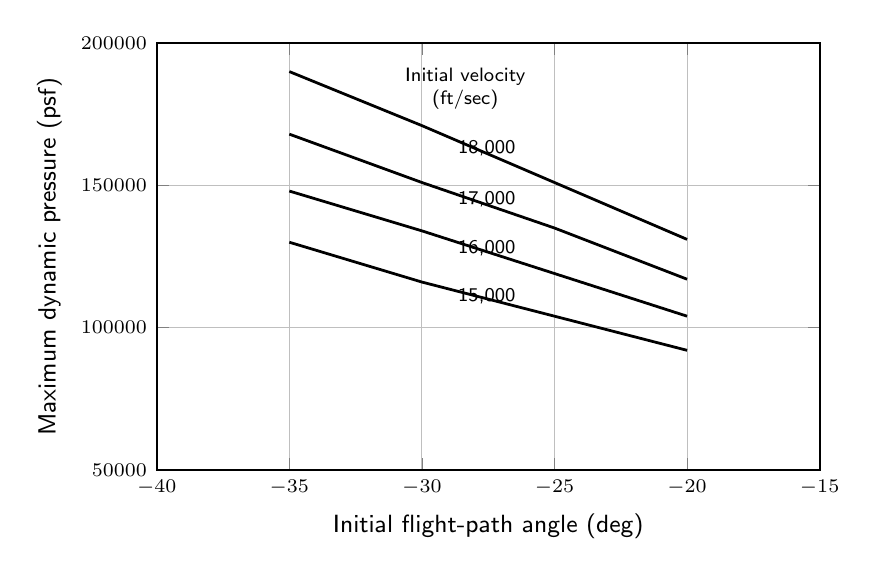
\begin{tikzpicture}
\begin{axis}[
  width=10.0cm,height=7.0cm,
  xmin=-40,xmax=-15,ymin=50000,ymax=200000,
  xtick={-40,-35,-30,-25,-20,-15},
  ytick={50000,100000,150000,200000},
  grid=major,
  axis line style={line width=0.8pt},
  tick label style={font=\scriptsize},
  label style={font=\sffamily\small},
  xlabel={Initial flight-path angle (deg)},
  ylabel={Maximum dynamic pressure (psf)},
  ylabel style={align=center},
  scaled y ticks=false,
  yticklabel style={/pgf/number format/fixed,/pgf/number format/1000 sep={}},
]
  \addplot[line width=1.0pt] coordinates {(-35,130000) (-30,116000) (-25,104000) (-20,92000)};
  \addplot[line width=1.0pt] coordinates {(-35,148000) (-30,134000) (-25,119000) (-20,104000)};
  \addplot[line width=1.0pt] coordinates {(-35,168000) (-30,151000) (-25,135000) (-20,117000)};
  \addplot[line width=1.0pt] coordinates {(-35,190000) (-30,171000) (-25,151000) (-20,131000)};
  \node[font=\sffamily\scriptsize,align=center,anchor=west] at (axis cs:-31,184000) {Initial velocity\\(ft/sec)};
  \node[font=\sffamily\scriptsize,anchor=west] at (axis cs:-29,163000) {18,000};
  \node[font=\sffamily\scriptsize,anchor=west] at (axis cs:-29,145000) {17,000};
  \node[font=\sffamily\scriptsize,anchor=west] at (axis cs:-29,128000) {16,000};
  \node[font=\sffamily\scriptsize,anchor=west] at (axis cs:-29,111000) {15,000};
\end{axis}
\end{tikzpicture}
